\inputencoding{utf8}
\chapter[Testiranje zmogljivosti Amazon EC2 platforme (P. Matičič, J. Pelicon, B. Rojc)]{Testiranje zmogljivosti Amazon EC2 platforme}

\pagestyle{fancy}
\fancyhf{}
\fancyhead[LE,RO]{\thepage}
\fancyhead[RE,LO]{\leftmark}

\huge Peter Matičič, Jan Pelicon, Blaž Rojc
\normalsize
\bigskip

\section{Opis problema}
V pričujočem razdelku opišite storitev, ki jo boste realizirali v obliki oblačne storitve in jo zmogljivostno analizirali. 

\section{Tehnična navodila za pisanje teksta}
Seminarsko nalogo v obliki pričujočega poglavja napišite v \LaTeX okolju. Številka vaše skupine vam bo dodeljena s strani prof. dr. Mraza. Najprej vaše poglavje poimenujte v datoteko "`poglavjeN"', kjer $N$ predstavlja dodeljeno številko. V nadaljevanju se na vse vire, slike, zapise itd. sklicujte s svojo številko. Vzorce najdete v nadaljevanju, kjer namesto vašega števila nastopa številka 1. Pravil se morate držati, da ne bomo imeli pri zlivanju poglavij v enotno delo preveč problemov.

Na vire se sklicujte z zapisom \cite{1_dOcean}, \cite{1_greenwade93}. Slike uvrščajte v tekst na naslednji način. Na sliki \ref{fig:1_osnovnaShema} je predstavljen primer storitve, pri čemer morajo biti vse slike v EPS formatu.
\begin{figure}[H]
    \centering
    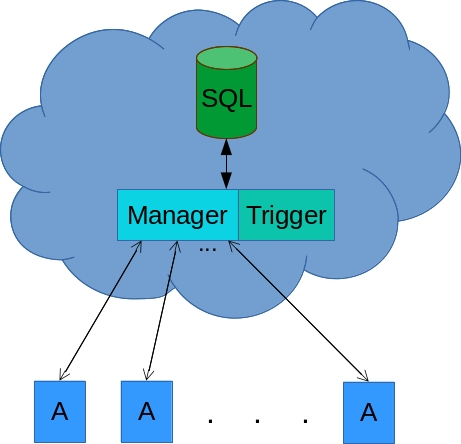
\includegraphics[scale=0.75]{Img/1_shema.jpg}
    \caption{Primer vstavitve slike v vaše poročilo.}
    \label{fig:1_osnovnaShema}
\end{figure}

Alineje naštevamo po naslednjem vzorcu:
\begin{itemize}
\item procesor: 1 jedro, Intel Xeon CPU E5-2650L v3 @ 1.8GHz,
\item ram: 1GB,
\item disk: 30GB.
\end{itemize}

V tabeli \ref{table:1_chunks} je prikazanih nekaj podatkov.
\begin{table}[H]
    \centering
        \begin{tabular}{ | r | r | r | r |} 
            \hline
           velikost koščkov & \textit{x} & \textit{y} & \textit{z} \\
            \hline
            Google Drive & 10 MB & 5 MB & 15 MB \\
            Mega & 1 MB & 0.5 MB & 1.5 MB \\
            \hline
        \end{tabular}
        \caption{Privzeta velikost koščkov \textit{x}, polovična privzeta velikost \textit{y} in za polovico povečana privzeta velikost \textit{z}.}
    \label{table:1_chunks}
\end{table}

Koda je predstavljena v izpisu \ref{lst:1_lst_cpu}.
\begin{lstlisting}[caption={Primer testiranja procesorja.}, label={lst:1_lst_cpu}]
zzrs@ZZRS:~$ sysbench --test=cpu --cpu-max-prime=20000 run
sysbench 0.4.12:  multi-threaded system evaluation benchmark

Running the test with following options:
Number of threads: 1

Doing CPU performance benchmark

Threads started!
Done.

Maximum prime number checked in CPU test: 20000


Test execution summary:
    total time:                          29.6635s
    total number of events:              10000
    total time taken by event execution: 29.6616
    per-request statistics:
         min:                                  2.55ms
         avg:                                  2.97ms
         max:                                 56.83ms
         approx.  95 percentile:               3.33ms

Threads fairness:
    events (avg/stddev):           10000.0000/0.00
    execution time (avg/stddev):   29.6616/0.00
\end{lstlisting}


\section{Zaklju"cek}
Tule bo zaključek.

\inputencoding{cp1250}